
\documentclass[12pt]{article}
\usepackage{graphicx} % for including images
\usepackage{hyperref} % for creating hyperlinks
\usepackage{amsmath} % for mathematical expressions
\usepackage{lipsum} % for generating dummy text
\usepackage{listings} % for code blocks
\usepackage{float} % place images where they appear in the LaTeX
\usepackage{pdfpages} % insert PDFs in the document

\lstset{
  language=bash,
  basicstyle=\ttfamily,
  breaklines=true
}

\begin{document}
% Title page information
\title{Does the Raspberry Pi 4B Have a GPGPU?}
\author{Jaidon Lybbert, University of Washington}
\date{January 24, 2024}

% Generate the title page
\maketitle

% Abstract section
\begin{abstract}
The Raspberry Pi 4B uses the Broadcomm BCM2711 SoC, which features a quad-core ARM Cortex-A72 CPU, and a Broadcomm VideoCore VI GPU. The VideoCore VI GPU is purpose-built for graphics applications, and there is very limited support for directly programming the device from the manufacturer. The focus of this article is to investigate the capabilities of the VideoCore GPU for General Purpose GPU (GPGPU) tasks, that is, compute tasks not involving graphics. Several open-source methods of programming are evaluated, and performance of the GPU is benchmarked against the CPU for the General Matrix Multiply (GEMM) algorithm extensively used in machine learning and machine vision applications.
\end{abstract}

% Introduction section
\section{Introduction}
This document is organized as follows. In Section \ref{sec:background} I describe where the VideoCore GPU sits in the context of the computing world, and introduce the most significant open-source efforts to program it. I explain the baselines we have to compare the VideoCore to, the benchmarks performed, and walk through the process of getting something to run on the GPU in Section \ref{sec:methods}. I show the benchmark results in Section \ref{sec:results}, and discuss the results and scaling in Section \ref{sec:discussion}. I conclude in \ref{sec:conclusion} by discussing the overall takeaways from my experiments and things I would like to try in the future.

% Methods section
\section{Background}\label{sec:background}

\subsection{GPUs and GPGPUs}
As clock rates stopped increasing, and Moore's law began to taper off, parallel processers emerged to increase compute throughput by allowing some algorithms to be broken down into pieces that could be solved simeoultaneously. Fueled by the \verb|$300B| gaming industry, parallel processors have rapidly taken over for video-encoding and decoding in computers and mobile phones. Nearly anything displaying to a screen now has a graphics processor. The emergence of AI training and inference has created new demand for General Purpose GPUs (GPGPUs) which are not restricted to graphics processing, but can be easily programmed for other compute tasks. NVIDIAs CUDA platform is built for this market, making programming their family of GPUs easy by providing a language, compiler, and debugging tools that integrate with existing languages and tools like C++, and Visual Studio.

Machine vision algorithms like Simultaneous Localization And Mapping (SLAM), and other applications, demand portable GPGPUs which can be programmed with arbitrary code and be integrated into a small portable device to perform parallel processing. The NVIDIA Jetson family of devices is tailored to this market, offering scaled down chips, and development boards for embedded programmers as low as \verb|$150|.

In this article, we will look at the GPU on the Raspberry Pi. A device which, as we'll see, was clearly not intended to be used as a GPGPU. However, recent developments in software drivers and graphics APIs just might enable this device to do useful compute workloads on the GPU. 

\subsection{VideoCore IV and VI}
The Broadcomm chips in the Raspberry Pis have VideoCore GPUs. The Raspberry Pi 1, 2, and 3 have the VideoCore IV GPU, and the Raspberry Pi 4 has the VideoCore VI GPU. The VideoCore IV is also found in devices such as the Roku, Amazon Fire TV Stick, and phones from Samsung, Nokia, and Apple's iPod. 

We will focus on the BCM2711 SoC featured in the Raspberry Pi 4B, which has a VideoCore VI GPU. 

\subsection{Motivation}
Two big questions motivate my research: ``what is the performance of the VideoCore VI GPU?'' and ``how do I program it?''

This small list of large questions breaks down into a large list of smaller questions.

\begin{itemize}
  \item What is the compute throughput of the VideoCore VI GPU?
  \item How do instructions map to hardware?
  \item How many parallel threads does the GPU support?
  \item What other APIs exist for GPU programming?
  \item Previous work done and results
  \item What is the memory model for the GPU + CPU?
  \item CPU and GPU caching?
  \item Supported language bindings?
  \item Memory latency?
\end{itemize}

\subsection{Prior Works}

Broadcomm has not released much documentation for the VideoCore VI GPU. Much of the information about the GPU is derived from the previous VideoCore IV reference manual \cite{videocoreiv}, which Broadcomm did release, and open-source drivers written with the help of Broadcomm engineers in the Linux kernel repository \cite{torvalds_linux_2024}, and the MESA graphics library \cite{external-mesa}. 

Various projects over the years have attempted to make programming the GPUs easier on the Raspberry Pi. 

The GitHub user ``hermanhermitage'' investigated the VideoCore IV GPU, and created a wiki their findings \cite{videocoreiv_herman}. They used US patent applications filed by Broadcomm along with experimentation to characterize the architecture, memory layout, instruction set, and registers for the device. The project includes a guide on intercepting GPU execution by replacing the \verb|bootcode.bin| in the boot partition of the SD card. Broadcomm eventually published a full specification for the VideoCore IV, superceding this effort with official documentation.

QPULib is a C++ library by Matthew Naylor for compiling and offloading programs for the VideoCore IV GPU (Raspberry Pi versions 1, 2, 3) during runtime \cite{QPULib}. Efforts by Wim Rijnders extended this idea to the VideoCore VI in the Raspberry Pi 4, with the C++ library V3DLib \cite{rijnders2021v3dlib}. V3DLib depends on the Mesa graphics library for disassembly of VideoCore instructions. It's worth noting that neither of these projects have had active development in the last 3 years, and support for new OS versions is unknown. 

A totally separate project, \verb|py-videocore6| \cite{pyvideocore6}, is a Python library enabling the programming of the VideoCore VI through the Direct Rendering Manager (DRM) graphics driver in the Linux kernel.

The Raspberry Pi Foundation recently announced that the Raspberry Pi 4 is now Vulkan 1.2 compliant through the Mesa graphics driver. This was a joint effort by Raspberry Pi, Mesa, and Broadcomm developers. Vulkan is a graphics library, which in contrast to older graphics libraries like OpenGL ES, supports an efficient compute-only pipeline, without any involvement of the framebuffer. Vulkan has been getting used more recently in machine learning applications for its cross-platform support. 

\section{Methods}\label{sec:methods}
\subsection{Setting the Baseline}
To evaluate the performance of the VideoCore VI GPU, there are two useful comparisons: 

\begin{itemize}
\item How does it perform compared to the CPU on-chip?
\item How does it perform compared to an NVIDIA Jetson?
\end{itemize}

The first question is arguably more relevant to someone who already has a Raspberry Pi. After all, why go through the trouble if the CPU is way faster anyway? 

\subsection{CPU GMEM Benchmarks}

As a benchmark, I chose to use a naive matrix multiply algorithm, as it's easy to implement and analyze. The algorithmic complexity is $O(n^3)$. For the basic CPU version, I use Bing AI to generate the algorithm in Rust which iterates over many matrix sizes, and records their execution times to a \verb|.csv| file. I then use Bing AI to generate a Python function to plot the results from the \verb|.csv| file. See the Appendix for Bing chat logs. From there, I debugged the boilerplate code with the help of the \textit{rust-analyzer} and \textit{pylsp} in my code editor, and modified it to my liking.

\subsection{Cortex-A72 Characterization}

The ARM Cortex-A72 CPU is thoroughly documented by ARM, with a public reference manual \cite{ARM2021}. Details specific to the Raspberry Pi 4B are published in the Raspberry Pi documentation \cite{raspberrypi2024}. The relevant high-level details are summarized here.

\subsubsection{CPU Architecture}

The Cortex-A72 CPU in the Raspberry Pi 4B has 4 cores, each with 32kB data cache and 48kB instruction cache. The cores share a 1MB L2 cache. The organization is shown in Fig \ref{fig:A72_arch}.

\begin{figure}[h]
\centering
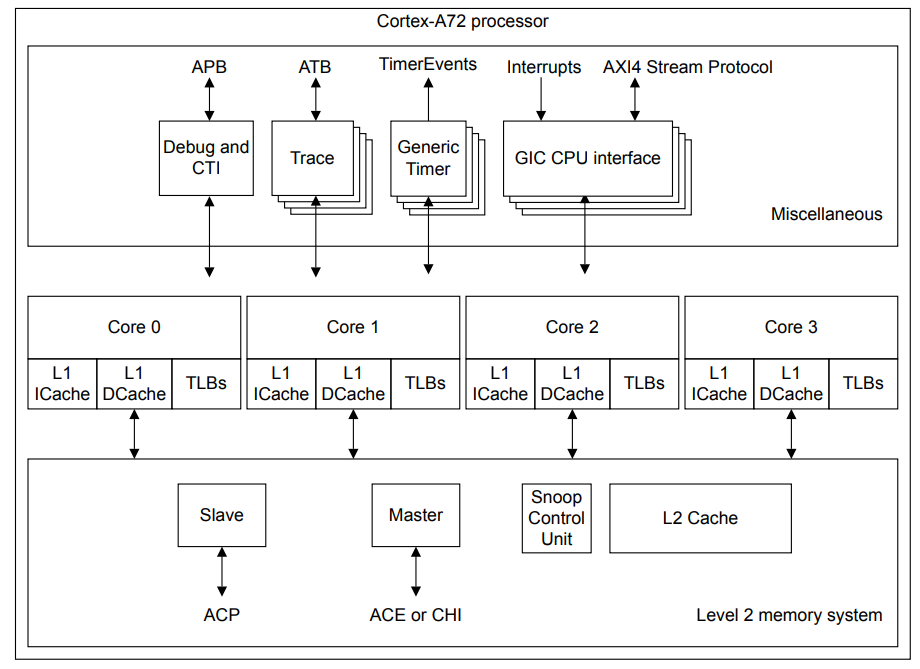
\includegraphics[width=1.0\textwidth]{A72_Core_Diagram.png} % replace with your own image file
\caption{Block diagram of the quad-core ARM Cortex-A72 CPU.}
\label{fig:A72_arch}
\end{figure}

The CPU supports SIMD operations through the Advanced SIMD and FP feature, has a Translation Lookaside Buffer (TLB), and has a module for prefetching memory, as shown in Fig \ref{fig:A72_fbd}. Using the 128-bit SIMD pipeline, for 4 cores it is theoretically possible to do 24 GFLOPS at 1.5GHz with single-precision.

\begin{figure}[h]
\centering
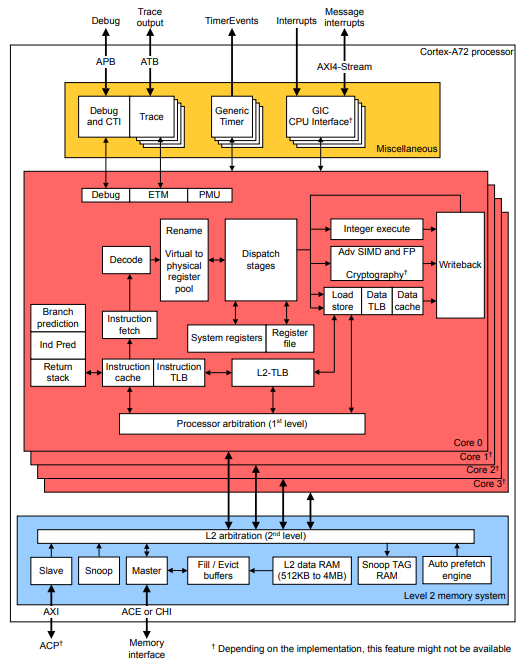
\includegraphics[width=0.5\textwidth]{A72_FBD.png} % replace with your own image file
\caption{Functional block diagram of the quad-core ARM Cortex-A72 CPU.}
\label{fig:A72_fbd}
\end{figure}

\subsubsection{Memory}

\begin{itemize}
\item 32kB data + 48kB instruction L1 cache per core
\item 1MB L2 cache
\end{itemize}

\subsection{VideoCore VI Characterization}

The VideoCore VI on the Raspberry Pi 4B is a 32-bit vector processor that operates on 16-element 32-bit integer or floating-point registers. These registers are 16-elements deep, meaning each register addresses 16 32-bit values. The processor is split into 8 Quad Processing Units (QPU), organized into two ``slices'' of 4 QPUs, which each have 4 physical cores Fig \ref{fig:v3d_core}. Each physical core contains an add ALU and a multiply-add ALU Fig \ref{fig:v3d_alus} \cite{rijnders2021v3dlib}. 

This puts the theoretical throughput of the device at 32 GFLOPS \cite{pyvideocore6}.

\begin{figure}[h]
\centering
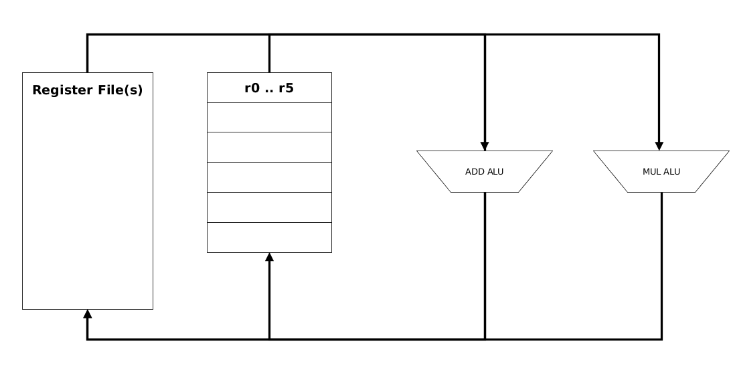
\includegraphics[width=1.0\textwidth]{v3d_alus.png} % replace with your own image file
\caption{Block diagram showing one physical core of the VideoCore processor.}
\label{fig:v3d_core}
\end{figure}

\begin{figure}[h]
\centering
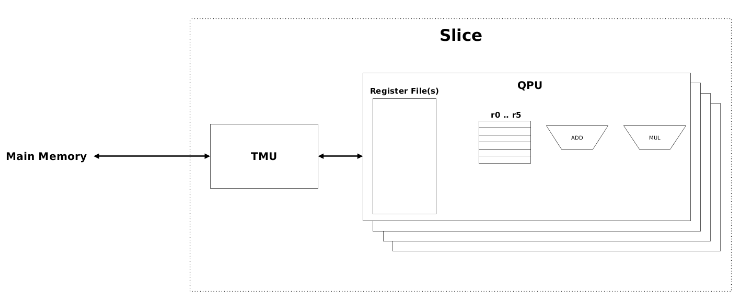
\includegraphics[width=1.0\textwidth]{v3d_core.png} % replace with your own image file
\caption{Block diagram showing the architecture of the VideoCore processor.}
\label{fig:v3d_alus}
\end{figure}

\subsection{Programming the VideoCore VI}

I found three open-source projects which could allow programming the VideoCore VI with compute workloads. I attempt to install each of them here.

\subsubsection{V3DLib}

V3DLib is a language and compiler for the VideoCore VI GPU created by Wim Rjinder's in C++. The project has a large number of dependencies, and ultimately uses the Mesa graphics library to translate code to run on the device. Because of the large number of dependencies and stale development (hasn't been updated in 3 years), it may be prohibitively difficult to use this method of programming. 

I cloned the repository and ran the build script.
	
\begin{lstlisting}
> sudo apt-get install git                                     
> sudo apt install libexpat1-dev                                
> git clone --depth 1 https://github.com/wimrijnders/V3DLib.git  
> cd V3DLib
> make QPU=1 DEBUG=1 all                                
\end{lstlisting}

The build failed due to missing headers, which I found were included in the raspberry pi development headers. I installed those, and the build failed again due to some XML parsing library missing. Since the build was taking a while, and it seemed like the project had long since been abandoned, I stopped here, to try the other options.

\subsubsection{pyvideocore6}

I followed the instructions in the GitHub repository to install the Python package.

\begin{lstlisting}
sudo usermod --append --groups video clusterpi
mkdir PyVideoCore
cd PyVideoCore
python3 -m venv venv
source venv/bin/activate
pip3 install setuptools wheel
git clone https://github.com/Idein/py-videocore6.git
cd py-videocore6/
python3 -m pip install --target sandbox/ --upgrade . nose

python3 setup.py build_ext --inplace
PYTHONPATH=sandbox/ python3 -m nose -v -s
\end{lstlisting}

The tests failed to run with the error message

\begin{lstlisting}
File "/home/clusterpi/PyVideoCore/py-videocore6/sandbox/nose/suite.py", line 106, in _set_tests
    if isinstance(tests, collections.Callable) and not is_suite:
                         ^^^^^^^^^^^^^^^^^^^^
AttributeError: module 'collections' has no attribute 'Callable'
\end{lstlisting}

I quickly found that `Callable' had been moved to `collections.abc.Callable' in newer versions of Python. To fix this I simply added this line to \verb|suite.py| under the import statements.

\begin{lstlisting}
collections.Callable = collections.abc.Callable
\end{lstlisting}

All tests then ran without issue. I then ran the SGEMM example. The results are shown in the next section.

\begin{lstlisting}
PYTHONPATH=sandbox/ python3 examples/sgemm.py
\end{lstlisting}

With more investigation, I discovered that the project developers had created a Basic Linear Algebra Subroutine (BLAS) library using this assembler. This project has more types of SGEMM implementations, among other algorithms. I attempted to install this BLAS library to test it out.

First I cloned and built the dependency.
\begin{lstlisting}
git clone https://github.com/Idein/libdrm_v3d
cd libdrm_v3d/
cmake .
make
ctest -V
\end{lstlisting}

The tests passed.

I then installed the package.

\begin{lstlisting}
make package
sudo dpkg -i libdrm_v3d_0.0.0_arm64.deb
\end{lstlisting}

I then compiled the BLAS library from the source repository, and ran the tests. The SGEMM results are shown in the next section.

\begin{lstlisting}
git clone https://github.com/Idein/qmkl6
cd qmkl6/
cmake .
sudo PYTHONPATH=~/PyVideoCore/py-videocore6/sandbox/ make
ctest -V
\end{lstlisting}

\subsubsection{Vulkan 1.2}

For my final test of programming the GPU, I will use the Vulkan 1.2 compliant Mesa graphics library driver. The Mesa driver for the VideoCore VI itself uses the Linux kernel V3D device driver to communicate with the device, just like \verb|py-videocore6| \cite{mesa3d}. In contrast to \verb|py-videocore6|, programming the GPU using the Vulkan 1.2 method uses the well-documented cross-platform Vulkan API instead of the one-off custom assembler that \verb|py-videocore6| uses. Since the Vulkan API is standard across all platforms, a wealth of knowledge and open-source exists for programming this way. To benchmark the device, I will use Google's \verb|uVkCompute| project. Which is described as ``a micro Vulkan compute pipeline and a collection of compute shaders for benchmarking/profiling purposes\cite{uVkCompute}.''

I started by downloading, compiling, and installing the latest Mesa driver (24.0.0) following the Mesa 3D documentation \cite{mesa3d}. I used GCC 12.2.0 and Python 3.11.2. I ran into many dependency issues, and found an article by Qengineering on building Mesa specifically for the Raspberry Pi 4. I used this guide as a reference \cite{q-engineering}. Some of the dependencies listed in the guide are no longer available on the default apt repository, and I simply skipped them.

At the install step of the guide, my process was slightly different.

\begin{lstlisting}
mkdir mesa
cd mesa
python -m venv venv
source venv/bin/activate
pip install meson mako
git clone -b 24.0 https://gitlab.freedesktop.org/mesa/mesa.git mesa_vulkan
cd mesa_vulkan

CFLAGS="-mcpu=cortex-a72" \
CXXFLAGS="-mcpu=cortex-a72" \
meson --prefix /usr \
-D platforms=x11 \
-D vulkan-drivers=broadcom \
-D gallium-drivers=kmsro,v3d,vc4 \
-D buildtype=release build

ninja -C build -j4
\end{lstlisting}

The build took about 45 minutes, and finished without error. I installed the binaries.

\begin{lstlisting}
sudo ninja -C build install
\end{lstlisting}

I originally intended to install the uVkCompute project from Google, but the installation process for the Vulkan SDK on the Raspberry Pi deterred me. The developers of Vulkan SDK provide an installer for x86 Linux, but don't have information on building for the \verb|aarch64| architecture. It is certainly possible to do, but the path is unclear. I instead opted to compile and test a sample project showcasing headless Vulkan from a popular set of Vulkan samples (137 contributers, 9.5k stars on GitHub) from Sascha Willems \cite{willems2024}. This project contains everything needed to build the sample projects with CMAKE and a compiler, including the Vulkan libraries. This is also used by the Q-engineering install guide \cite{q-engineering} so I knew it would work.

\begin{lstlisting}
git clone --recursive https://github.com/SaschaWillems/Vulkan.git
cd Vulkan
mkdir build
cd build
cmake -DCMAKE_BUILD_TYPE=Release ..
make -j4
\end{lstlisting}

The project took about 10 minutes to build with no errors. I then ran the headless compute example. This example computes a fibonacci sequence in the Vulkan compute shader on the GPU and returns the results to the shell output.

\begin{lstlisting}
cd bin
./computeheadless
\end{lstlisting}

The program ran successfully with the output in Fig \ref{fig:computeheadless}, validating Vulkan as a method of programming the Raspberry Pi 4B GPU. 

\begin{figure}[h]
\centering
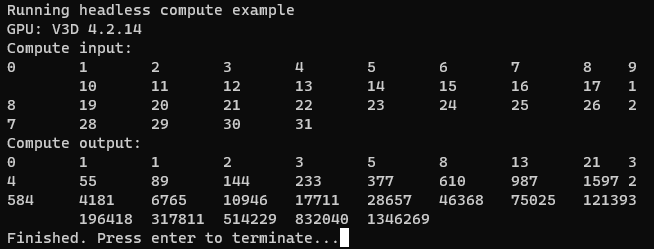
\includegraphics[width=1.0\textwidth]{Headless_Compute.png} % replace with your own image file
\caption{Output of the headlesscompute Vulkan sample from Sascha Willems, running on the Raspberry Pi 4B through the Mesa graphics library driver.}
\label{fig:computeheadless}
\end{figure}

% Results section
\section{Results}\label{sec:results}

\subsection{CPU GEMM Performance}
I implemented a naive GEMM algorithm in Rust, and compared my implementation to the Numpy implementation, which uses all cores and the SIMD engine. The difference was outstanding. See Fig \ref{fig:gemm}, \ref{fig:gemm_numpy}. My implementation was orders of magnitude slower. In the time my Rust implementation multiplied two 200x200 matrices, Numpy could do two 2000x2000 matrices. This is particularly impressive considering the $O(N^3)$ complexity of the algorithm. The Numpy algorithm equates to 8 GFLOPS, while my Rust algorithm performs at just 8 MFLOPS. 

\begin{figure}[h]
\centering
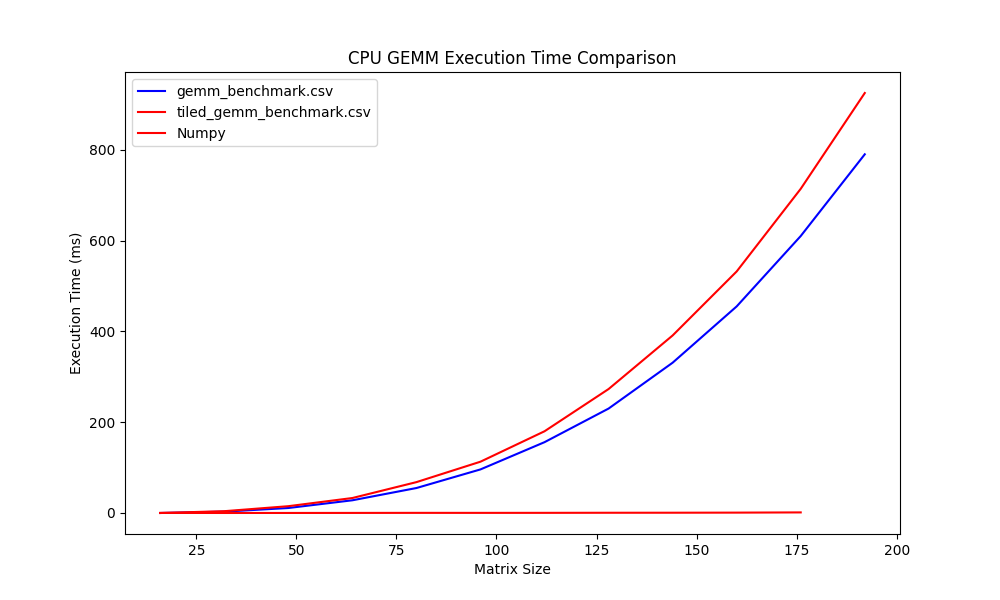
\includegraphics[width=1.0\textwidth]{gemm.png} % replace with your own image file
\caption{Comparison of 3 CPU GEMM implementations, the slow ones are mine implemented in Rust. The Numpy implementation is the ``@'' operator in the Python library Numpy.}
\label{fig:gemm}
\end{figure}

\begin{figure}[h]
\centering
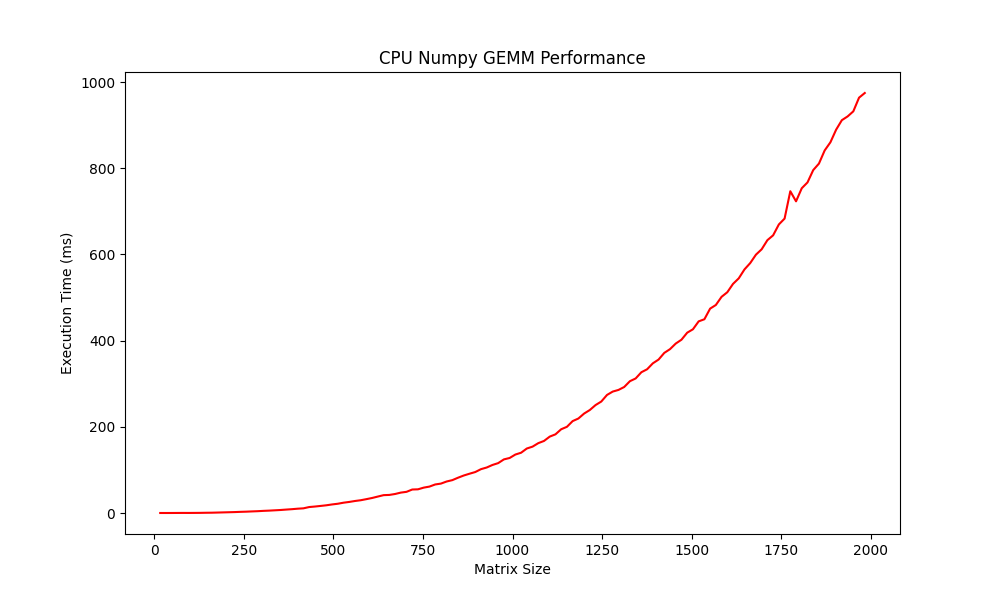
\includegraphics[width=1.0\textwidth]{gemm_numpy.png} % replace with your own image file
\caption{Numpy CPU implementation of GEMM using the all cores and the SIMD engine of the A72.}
\label{fig:gemm_numpy}
\end{figure}

\subsection{GPU Theoretical Comparison to the CPU}
The CPU and GPU share memory on chip, the performance differences will come down to how well they cache and manage memory and their throughput. I will ignore the memory considerations, and simply compare their theoretical compute throughput to get a ballpark estimate of how they compare. Although the VideoCore does have cache, it is unkown how much, since that information is not published.

\begin{center}
\begin{tabular}{|l|c|c|}
\hline
Property & VideoCore VI & ARM A72 \\
\hline
FLOPS & 32 GFLOPS & 24 GFLOPS \\
\hline
\end{tabular}
\end{center}

\subsection{GPU Benchmark Comparison to CPU}
I used the py-videocore6 SGEMM test to compare CPU and GPU performance.

\begin{lstlisting}
==== sgemm example (1024x1024 times 1024x1024) ====
numpy: 0.0961 sec, 22.38 Gflop/s
QPU:   0.5735 sec, 3.75 Gflop/s
Minimum absolute error: 0.0
Maximum absolute error: 0.0003814697265625
Minimum relative error: 0.0
Maximum relative error: 0.13134673237800598
\end{lstlisting}

These GPU results are consistent with the test results reported by the project developers, but in their case, Numpy had similar performance to the GPU. It would seem that the Numpy library has been updated since then, using the SIMD hardware of the Cortex-A72 to speed up the matrix multiply, and achieve very near the theoretical peak performance.

I also tried the qmlk6 BLAS library implementation of SGEMM.

The peak throughput of the GPU during the qmlk6 SGEMM tests reached 5.8 GFLOPs, Fig \ref{fig:qpu_blas}. 

\begin{figure}[h]
\centering
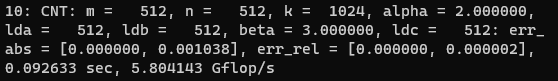
\includegraphics[width=1.0\textwidth]{QPU_BLAS_Peak.png} % replace with your own image file
\caption{Best compute throughput results from running the qmkl6 tests. The meaning of the various parameters are common usages in BLAS libraries. In this case we are multiplying a 512x1024 matrix A by a 1024x512 matrix B to produce a 512x512 result C. The parameters lda, ldb, ldc refer to the ``leading dimension of [a, b, c].''}
\label{fig:qpu_blas}
\end{figure}

\subsection{Theoretical Comparison to NVIDIA Jetson Nano}
In order to make meaningful observations about the capability of the Broadcomm VideoCore VI GPU on the Raspberry Pi 4B, I will compare the programming experience and capabilities of the device to the widely used NVIDIA CUDA platform. Obviously, with the NVIDIA devices being more expensive, they have many more cores and features, but on a core-to-core basis they are similar SIMD processors with similar function. For comparisons sake, I will show how the \verb|$35| 2GB Raspberry Pi 4B \textbf{theoretically} stacks against the \verb|$150| NVIDIA Jetson Nano device.

\subsubsection{Hardware}
\begin{center}
\begin{tabular}{|l|c|c|}
\hline
Property & Raspberry Pi 4B & Jetson Nano \\
\hline
GPU & Broadcomm VideoCore VI & 128-core NVIDIA Maxwell \\
\hline
CPU & Quad-core ARM A72 & Quad-core ARM A57  \\
\hline
Memory & 4GB LPDDR4 & 4GB LPDDR4 \\
\hline
Memory Bandwidth & 12.8GB/s & 25.6GB/s \\
\hline
GPU GFLOPS & 32 & 472 \\
\hline
Power Usage (W) & 3.4 | 7.6 & 5 | 10 \\
\hline
Cost & \$35 & \$130 \\
\hline
\end{tabular}
\end{center}

\paragraph{Note}
\textit{Values are taken from Raspi documentation \cite{raspberrypi2024}, published benchmarks \cite{Zwetsloot2024}, and the NVIDIA product page \cite{jetsonstore}}

\subsubsection{Software}

\paragraph{NVIDIA}
NVIDIA provides proprietary drivers, the CUDA language, the NVCC compiler, the NSIGHT debugger, and profiling tools with NSIGHT Systems. Their drivers are compliant with OpenCL, Vulkan, and OpenGL standards. There is a large amount of open-source example code provided by NVIDIA for using these APIs, and interoperability. There is CUDA integration in the most well-known ML libraries like TensorFlow and PyTorch. 

\paragraph{VideoCore}
Broadcomm doesn't provide any device driver for the VideoCore GPU. They officially published the specification for the VideoCore IV, but never the VI or VII in the Pi 4 and 5. All software libraries I have found ultimately communicate with the VideoCore through the Linux kernel V3D DRM device driver, which supports OpenGL ES. The open-source Mesa device driver is a wrapper around the DRM driver for the VideoCore VI and recently became Vulkan 1.2 compliant. Software development for programming the GPU outside of graphics is sparse and outdated. The options are to either program the GPU with a custom open-source assembler maintained by 1 person, or install the Mesa driver and program it using Vulkan compute shaders. No working language, debugger, or profiling tool exists as far as I can tell.

\paragraph{Verdict}
NVIDIA wins the battle in the world of software for GPGPU development, and it's not even close. The VideoCore GPU, true to its name, was designed for video and graphics, and Broadcomm never intended for it to be used for GPGPU tasks.

% Discussion section
\section{Discussion}\label{sec:discussion}
\subsection{Cortex-A72 vs VideoCore VI}
While the theoretical 32 GFLOPs compute throughput of the VideoCore VI is higher than the 24GFLOPs of the A72, in practice, directly programming the VideoCore VI through py-videocore6 or qmkl6 resulted in SGEMM performance that was not even 1/6 the theoretical performance, while the Numpy CPU implementation very nearly achieved the theoretical peak of 24GFLOPS. Ultimately, the GPU was at best capable of 1/4 the compute throughput of the CPU.

\subsection{Raspberry Pi 4B vs Jetson Nano}

\subsubsection{Performance}
The Raspberry Pi 4B and Jetson Nano both feature a Quad-core ARM CPU, and 4GB LDDR4 for the models and price point chosen. The Jetson Nano claims double the memory bandwidth compared to the benchmarked Raspberry Pi 4B results, but I couldn't find any true benchmarks for the Nano. The power usage is slightly higher for the Nano.

The benchmarks show that the practical compute throughput of the VideoCore VI is about 5.8GFLOPS at best, and usually much lower. This pales in comparison to the theoretical 472 GFLOPS the Jetson Nano is capable of.  If we assume that both devices are running compute-bound workloads like the SGEMM (a poor assumption), so that memory access time isn't a bottleneck, the Nano outperforms the Pi 4B by a factor of 81.4, while being 4.2x the cost. 

\paragraph{The Real World of Memory-bound Workloads}
In reality, workloads are not compute-bound in general. One metric to analyze how much an algorithm is compute or memory-bound is the \textbf{arithmetic intensity} of the algorithm defined as the ratio of arithmetic operations to memory loads and stores. Algorithms are designed to be ideally compute-bound by maximizing the number of arithmetic operations and minimizing the number of memory operations. Despite incredible efforts optimizing memory access patterns, it is actually quite rare to achieve the compute-bound case. 

The general matrix-multiply (GEMM) algorithm is incredibly useful, and is great for GPUs because it can be made to have good arithmetic intensity, and be compute-bound with fast memory and good caching. In the ideal case with infinite cache, given an NxN matrix, for $2N^2$ memory reads, you perform $N^3$ arithmetic operations for an arithmetic intensity $N/2$, so the best case is very large matrices. In practice, this value must be much much greater than ratio of memory latency to the time it takes to do one arithmetic operation in order for the workload to be compute-bound. And of course, cache is not infinite.

All this is to say that the compute throughput of the NVIDIA Nano only really means anything if you're doing specific algorithms like AI training or machine vision, and little to nothing if you're talking about serving web requests.

\paragraph{At Scale}
If we look at a compute cluster made up of 400 Raspberry Pi 4Bs and compare to another made of 100 Nvidia Jetson Nanos, each slaving away training a neural net by doing a bunch of very large SGEMMs, the comparison would look something like the table below.

\begin{center}
\begin{tabular}{|l|c|c|}
\hline
Property & Pi Cluster & Nano Cluster \\
\hline
Nodes & 400 & 100 \\
\hline
GPU & Broadcomm VideoCore VI & 128-core NVIDIA Maxwell \\
\hline
CPU & Quad-core ARM A72 & Quad-core ARM A57  \\
\hline
Memory & 1.6TB LPDDR4 & 400GB LPDDR4 \\
\hline
Memory Bandwidth & 5.12TB/s & 2.56TB/s \\
\hline
GPU TFLOPS & 2.32 & 47.2 \\
\hline
CPU TFLOPS & 9.6 & 2.4\\
\hline
Total TFLOPS & 11.2 & 49.6\\
\hline
Power Usage (kW) & 1.3 | 3.0 & 0.5 | 1.0 \\
\hline
Cost & \$14k & \$15k \\
\hline
\end{tabular}
\end{center}

At scale, the Pi cluster begins to look like less of a machine-learning cluster, and more like a data or web server. The strengths of the Pi is the cheap access to a large number of processors and RAM, while the Nano would perform massively better for AI workloads.

\subsubsection{Programming}
The qmkl6 BLAS library performed well compared to the py-videocore6 example. The BLAS library abstracts away the assembly instructions needed to use the py-videocore6 assembler to program the device, and can be called directly from C++ code. \verb|qmkl6| is also easier to install and more lightweight than Vulkan. It would be my preferred method of programming using the GPU if I were to do single-platform compute-only tasks consisting only of BLAS routines. There are some minor issues installing the project due to no maintainence.

Mesa was a significant effort to install and requires a large amount of dependencies and disk space to get going. The benefit of Mesa is enabling Vulkan as a standard cross-platform API, which can also be used for graphics. Vulkan would generally be my preffered choice for programming the VideoCore, for the cross-platform code, and interoperability with graphics. By enabling Vulkan, the programming experience vastly improves in reliability and wealth of knowledge and open-source implementations of algorithms online.

% Conclusion section
\section{Conclusion}\label{sec:conclusion}
So, does the Raspberry Pi 4B have a GPGPU? Clearly, the answer is no. There is no support from the manufacturer for programming the GPU directly. What does exist is a few stagnant open-source projects made by a very few curious people who reverse-engineered the device from patent filings, disassembling OpenGL ES shader code, and inferring details from benchmarking and overdue specifications from previous generation chips. The GPU is slower than 1/4 the speed of the A72 using SIMD at the GEMM algorithm. Everything points to leaving the GPU for graphics tasks, which it has specialized hardware for.

However, there may still be value in using this VideoCore chip as if it were a GPGPU for select applications. After all, you have an entirely separate vector processor on the device capable of GFLOPs, why not use it if it's easy enough? Maybe there is some long running process that you can offload to your GPU to leave the CPU free for other tasks. Something that comes to mind is SLAM bundle adjustment. Bundle adjustment is an optimization step that executes on a large matrix of collected keypoints. It isn't time-critical like instantaneous pose-estimation, so it is okay to take seconds or minutes to perform. Offloading this algorithm to the GPU would free the CPU to service control interrupts and rapidly compute pose-estimation. 

\paragraph{Note}
\textit{All my code and project files for this and future reports, can be found on my GitHub repository \cite{lybbert2024classwork}.}

% Bibliography from refs.bib
\bibliographystyle{plain}
\bibliography{refs}

\section{Appendix: Bing Chat Log}
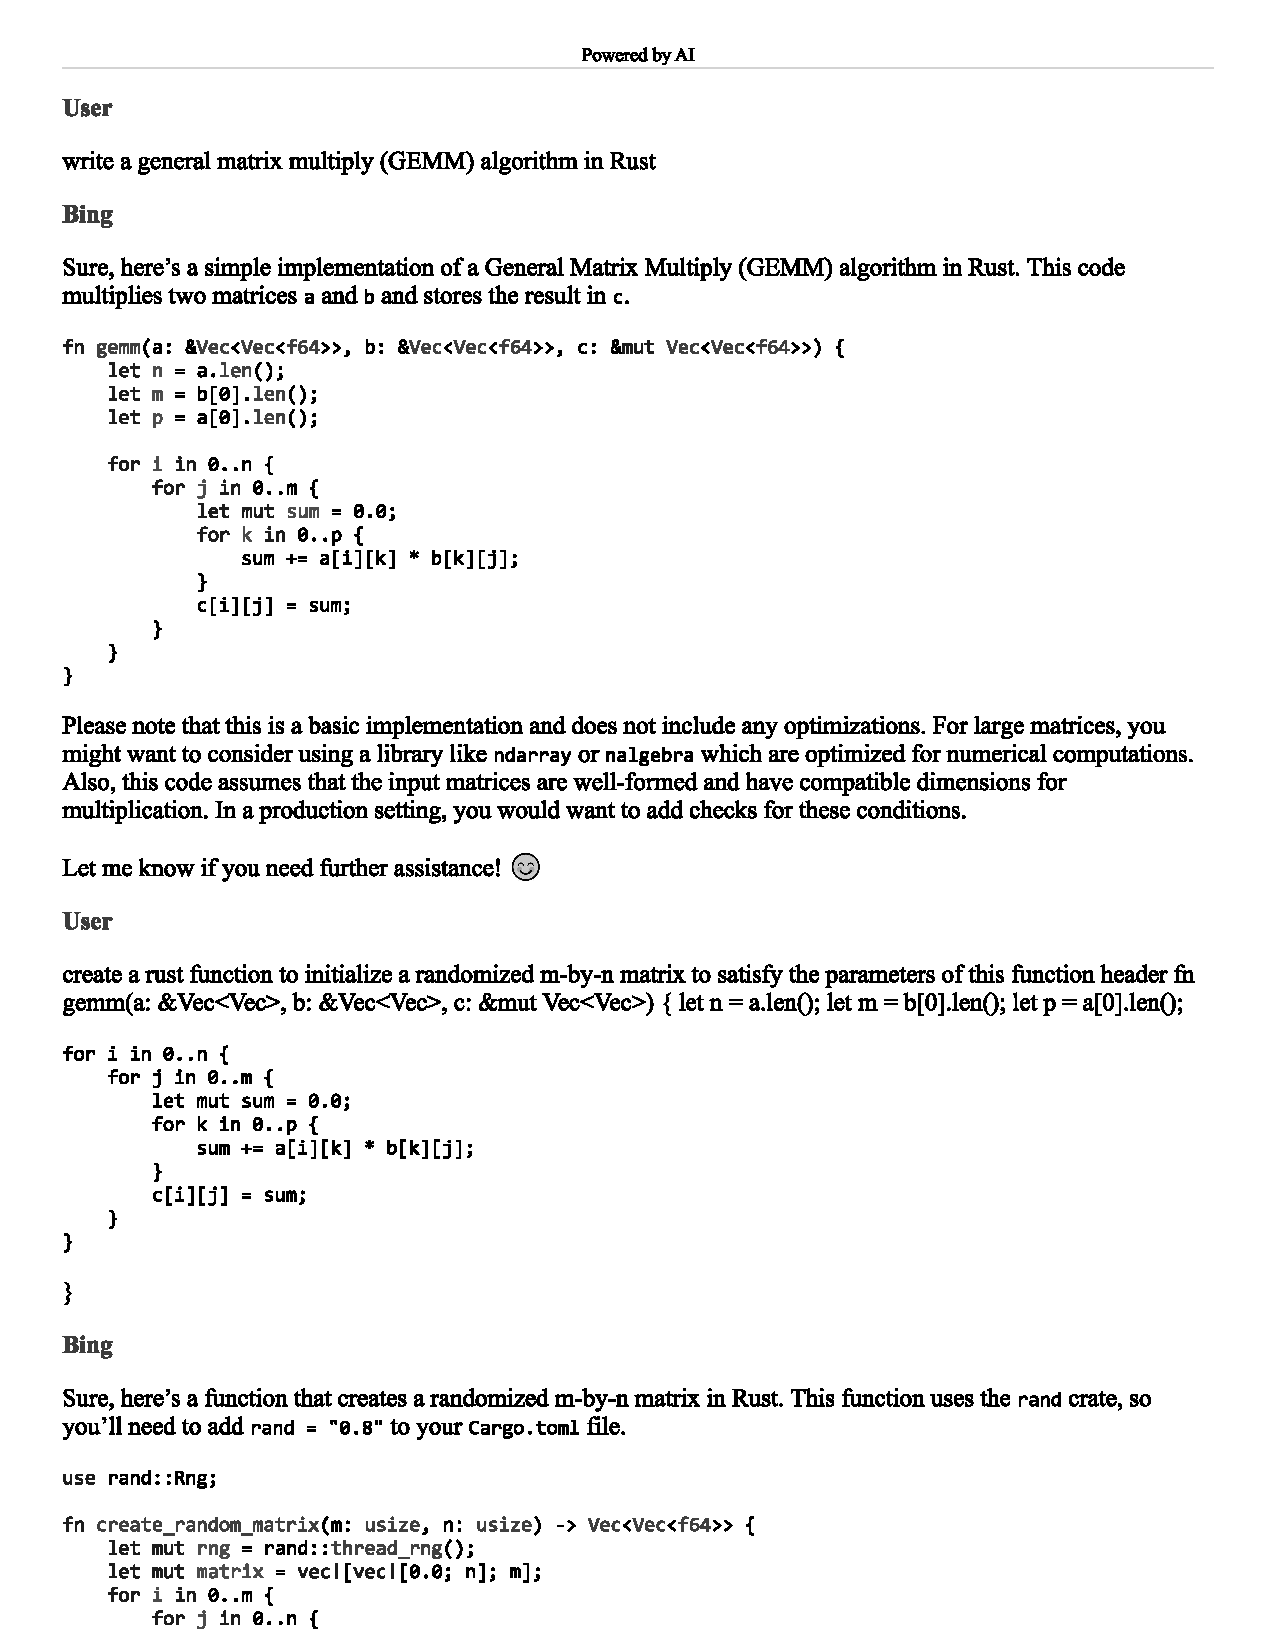
\includepdf[pages=-]{BingLog.pdf}

\end{document}
